% Template for PLoS
% Version 3.5 March 2018
%
% % % % % % % % % % % % % % % % % % % % % %
%
% -- IMPORTANT NOTE
%
% This template contains comments intended 
% to minimize problems and delays during our production 
% process. Please follow the template instructions
% whenever possible.
%
% % % % % % % % % % % % % % % % % % % % % % % 
%
% Once your paper is accepted for publication, 
% PLEASE REMOVE ALL TRACKED CHANGES in this file 
% and leave only the final text of your manuscript. 
% PLOS recommends the use of latexdiff to track changes during review, as this will help to maintain a clean tex file.
% Visit https://www.ctan.org/pkg/latexdiff?lang=en for info or contact us at latex@plos.org.
%
%
% There are no restrictions on package use within the LaTeX files except that 
% no packages listed in the template may be deleted.
%
% Please do not include colors or graphics in the text.
%
% The manuscript LaTeX source should be contained within a single file (do not use \input, \externaldocument, or similar commands).
%
% % % % % % % % % % % % % % % % % % % % % % %
%
% -- FIGURES AND TABLES
%
% Please include tables/figure captions directly after the paragraph where they are first cited in the text.
%
% DO NOT INCLUDE GRAPHICS IN YOUR MANUSCRIPT
% - Figures should be up\textit{loaded} separately from your manuscript file. 
% - Figures generated using LaTeX should be extracted and removed from the PDF before submission. 
% - Figures containing multiple panels/subfigures must be combined into one image file before submission.
% For figure citations, please use "Fig" instead of "Figure".
% See http://journals.plos.org/plosone/s/figures for PLOS figure guidelines.
%
% Tables should be cell-based and may not contain:
% - spacing/line breaks within cells to alter layout or alignment
% - do not nest tabular environments (no tabular environments within tabular environments)
% - no graphics or colored text (cell background color/shading OK)
% See http://journals.plos.org/plosone/s/tables for table guidelines.
%
% For tables that exceed the width of the text column, use the adjustwidth environment as illustrated in the example table in text below.
%
% % % % % % % % % % % % % % % % % % % % % % % %
%
% -- EQUATIONS, MATH SYMBOLS, SUBSCRIPTS, AND SUPERSCRIPTS
%
% IMPORTANT
% Below are a few tips to help format your equations and other special characters according to our specifications. For more tips to help reduce the possibility of formatting errors during conversion, please see our LaTeX guidelines at http://journals.plos.org/plosone/s/latex
%
% For inline equations, please be sure to include all portions of an equation in the math environment.  For example, x$^2$ is incorrect; this should be formatted as $x^2$ (or $\mathrm{x}^2$ if the romanized font is desired).
%
% Do not include text that is not math in the math environment. For example, CO2 should be written as CO\textsubscript{2} instead of CO$_2$.
%
% Please add line breaks to long display equations when possible in order to fit size of the column. 
%
% For inline equations, please do not include punctuation (commas, etc) within the math environment unless this is part of the equation.
%
% When adding superscript or subscripts outside of brackets/braces, please group using {}.  For example, change "[U(D,E,\gamma)]^2" to "{[U(D,E,\gamma)]}^2". 
%
% Do not use \cal for caligraphic font.  Instead, use \mathcal{}
%
% % % % % % % % % % % % % % % % % % % % % % % % 
%
% Please contact latex@plos.org with any questions.
%
% % % % % % % % % % % % % % % % % % % % % % % %

\documentclass[10pt,letterpaper]{article}
\usepackage[top=0.85in,left=2.75in,footskip=0.75in]{geometry}

% customized packages
\usepackage{fixltx2e}
\usepackage{stfloats}
\usepackage{subfloat}
\usepackage[caption=false,font=footnotesize]{subfig}

% amsmath and amssymb packages, useful for mathematical formulas and symbols
\usepackage{amsmath,amssymb}
% algorithm,algorithmicx,algpseudocode are used for writing pseudo code and algorithms
\usepackage{algorithm,algorithmicx,algpseudocode}
% multirow is used for adjusting the table
\usepackage{multirow}
% Use adjustwidth environment to exceed column width (see example table in text)
\usepackage{changepage}

% Use Unicode characters when possible
\usepackage[utf8x]{inputenc}

% textcomp package and marvosym package for additional characters
\usepackage{textcomp,marvosym}

% cite package, to clean up citations in the main text. Do not remove.
\usepackage{cite}

% Use nameref to cite supporting information files (see Supporting Information section for more info)
\usepackage{nameref,hyperref}

% line numbers
\usepackage[right]{lineno}

% ligatures disabled
\usepackage{microtype}
\DisableLigatures[f]{encoding = *, family = * }

% color can be used to apply background shading to table cells only
\usepackage[table]{xcolor}
\usepackage{booktabs}
% stop disconnecting vertical lines:
\setlength{\aboverulesep}{0ex}
\setlength{\belowrulesep}{0ex}
% array package and thick rules for tables
\usepackage{array}

% create "+" rule type for thick vertical lines
\newcolumntype{+}{!{\vrule width 2pt}}

% create \thickcline for thick horizontal lines of variable length
\newlength\savedwidth
\newcommand\thickcline[1]{%
	\noalign{\global\savedwidth\arrayrulewidth\global\arrayrulewidth 2pt}%
	\cline{#1}%
	\noalign{\vskip\arrayrulewidth}%
	\noalign{\global\arrayrulewidth\savedwidth}%
}

% \thickhline command for thick horizontal lines that span the table
\newcommand\thickhline{\noalign{\global\savedwidth\arrayrulewidth\global\arrayrulewidth 2pt}%
	\hline
	\noalign{\global\arrayrulewidth\savedwidth}}


% Remove comment for double spacing
%\usepackage{setspace} 
%\doublespacing

% Text layout
\raggedright
\setlength{\parindent}{0.5cm}
\textwidth 5.25in 
\textheight 8.75in

% Bold the 'Figure #' in the caption and separate it from the title/caption with a period
% Captions will be left justified
\usepackage[aboveskip=1pt,labelfont=bf,labelsep=period,justification=raggedright,singlelinecheck=off]{caption}
\renewcommand{\figurename}{Fig}

% Use the PLoS provided BiBTeX style
\bibliographystyle{plos2015}

% Remove brackets from numbering in List of References
\makeatletter
\renewcommand{\@biblabel}[1]{\quad#1.}
\makeatother



% Header and Footer with logo
\usepackage{lastpage,fancyhdr,graphicx}
\usepackage{epstopdf}
\graphicspath{{../Figures/}}
%\pagestyle{myheadings}
\pagestyle{fancy}
\fancyhf{}
%\setlength{\headheight}{27.023pt}
%\lhead{\includegraphics[width=2.0in]{PLOS-submission.eps}}
\rfoot{\thepage/\pageref{LastPage}}
\renewcommand{\headrulewidth}{0pt}
\renewcommand{\footrule}{\hrule height 2pt \vspace{2mm}}
\fancyheadoffset[L]{2.25in}
\fancyfootoffset[L]{2.25in}
\lfoot{\today}

%% Include all macros below

\newcommand{\lorem}{{\bf LOREM}}
\newcommand{\ipsum}{{\bf IPSUM}}

%% END MACROS SECTION


\begin{document}
	\vspace*{0.2in}

		{\Large\textbf\newline{{Supporting Document for Studied Specific Cases}} % Please use "sentence case" for title and headings (capitalize only the first word in a title (or heading), the first word in a subtitle (or subheading), and any proper nouns).
		}

\section*{Case Study}
%TODO: Add general discussion and motivate about the reason of conducting these case studies.
We conducted four different case studies to get more insight into the performance of assistive devices that include studying both assistive devices in a particular load condition or an assistive device in two different load conditions with the same effect on the metabolic energy expenditure or the same energy consumption of assistive actuators. Investigating these specific configurations of the optimal devices helped us to understand how the profiles of devices with the same performances are changing in a load condition more systematically. These cases can clarify the effect of load condition on an assistive device profiles, and their muscles and how a particular device will be affected by loading assisted subjects with a heavy load.
\begin{figure*}[!ht]   
	\centering
	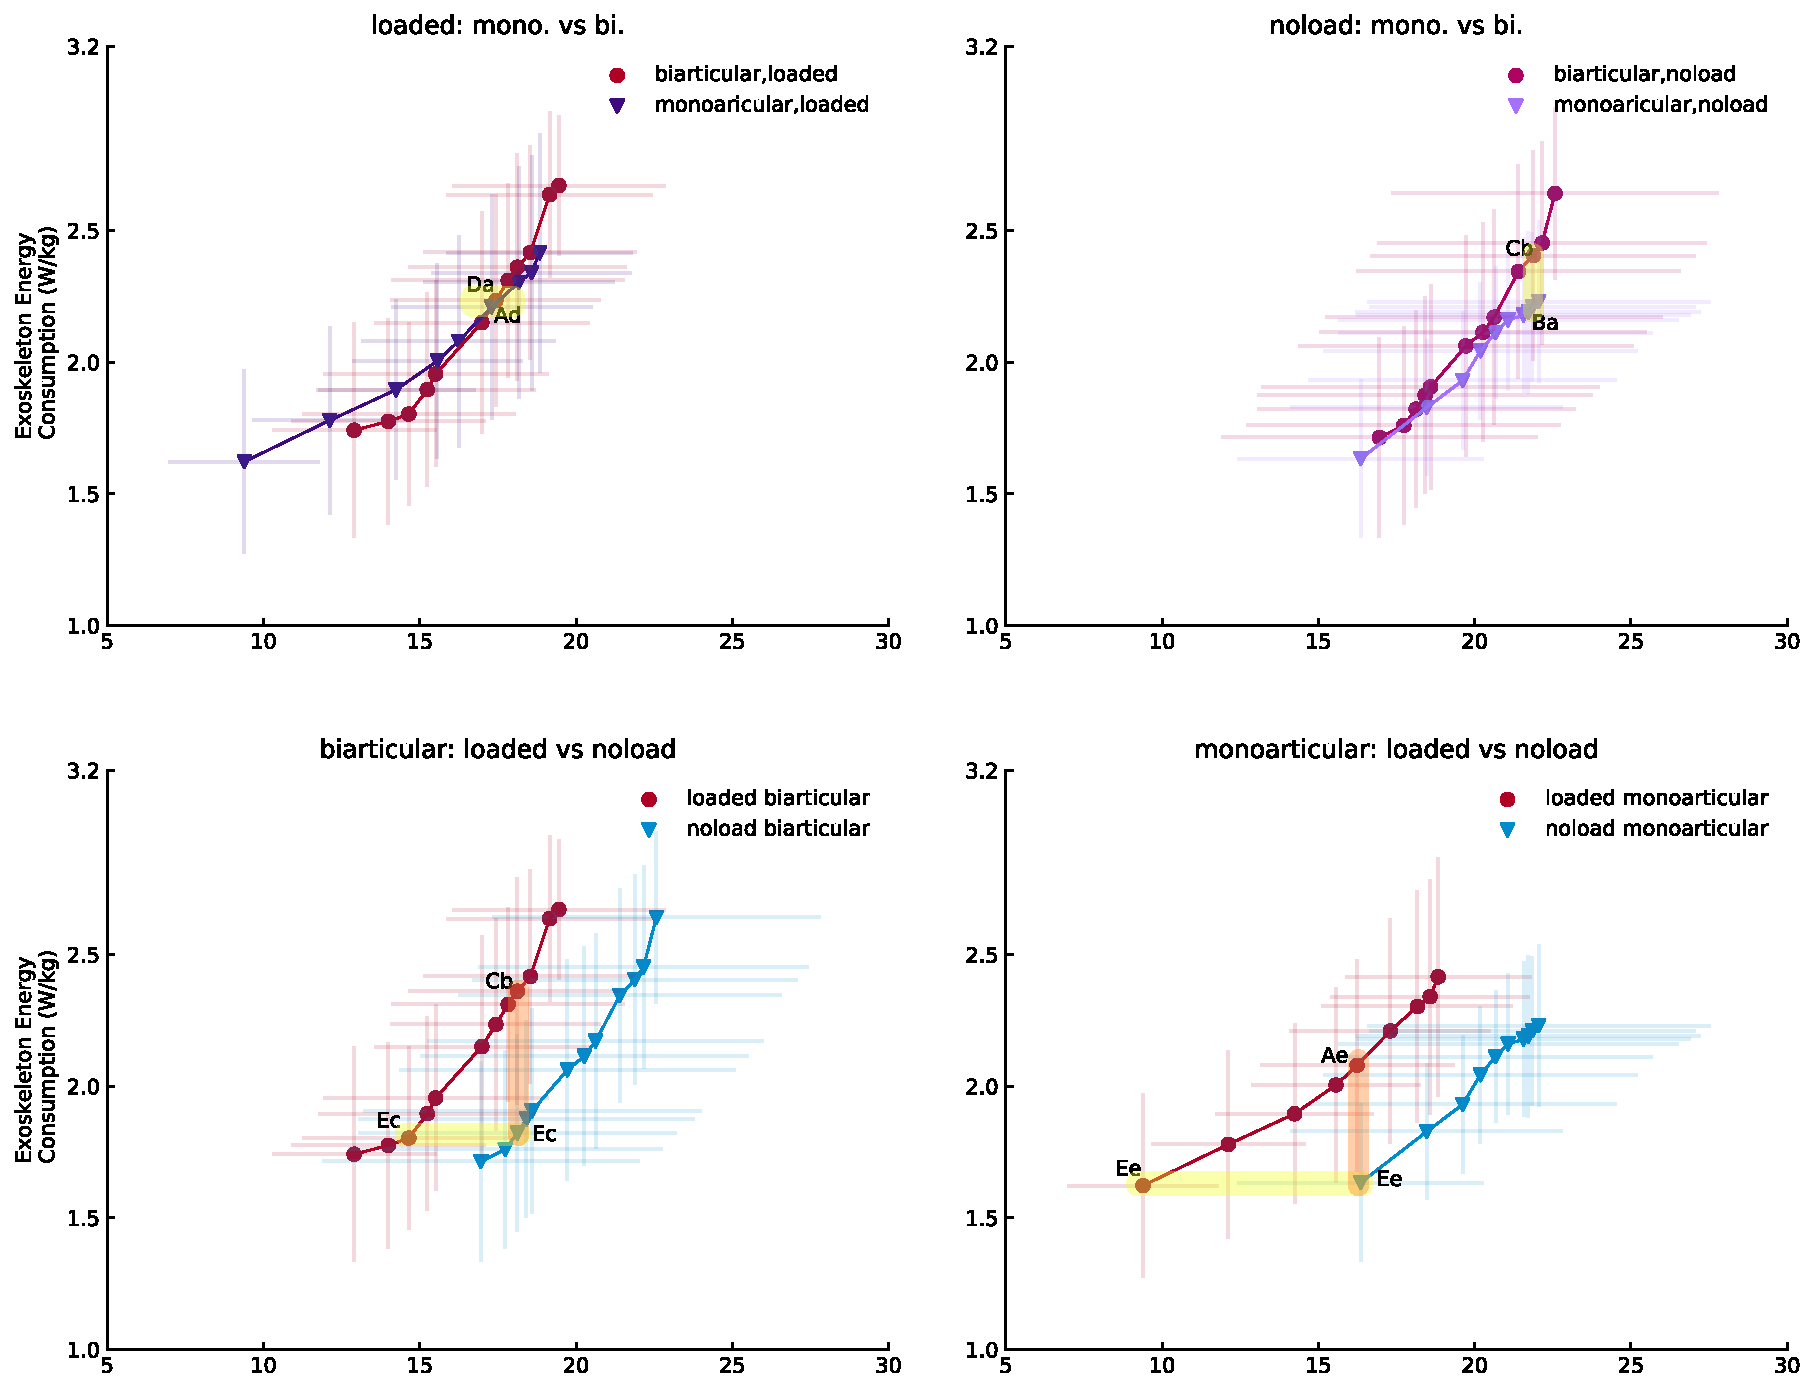
\includegraphics[width=\linewidth]{Case_Studies/PaperFigure_Selected_Configurations.pdf}
	\vspace{1mm}
	\caption{{\small\textbf{Optimal trade-offs between metabolic cost reduction and device energy consumption.} The optima points on Paretofronts are resulted from averaging over 7 subjects.}}
	\label{Fig_Selected_OptimalDevices_On_Pareto}
\end{figure*}
\subsubsection*{Case 1: Devices Performance in \textit{\textit{loaded}} Condition}
It is shown that the optimal trade-offs of both exoskeletons are practically the same for {\it loaded} condition, and due to this issue, we selected two devices on Pareto front that have almost the same performance in both metabolic cost reduction and power consumption. The chosen device for monoarticular has 70 N.m hip peak torque and 40 N.m knee peak torque, which is represented by "$Ad$ " on Pareto front ( figure \ref{Fig_Main_Paretofronts}) and the peak torques of the biarticular device are 40, and 70 N.m on hip and knee respectively represented with "$Da$ " on the Pareto front. As it can be inferred from the configurations of devices, although these two devices have the same performance on defined objectives, they have a completely different arrangement on hip and knee actuators.
\begin{figure*}[ht]   
	\centering
	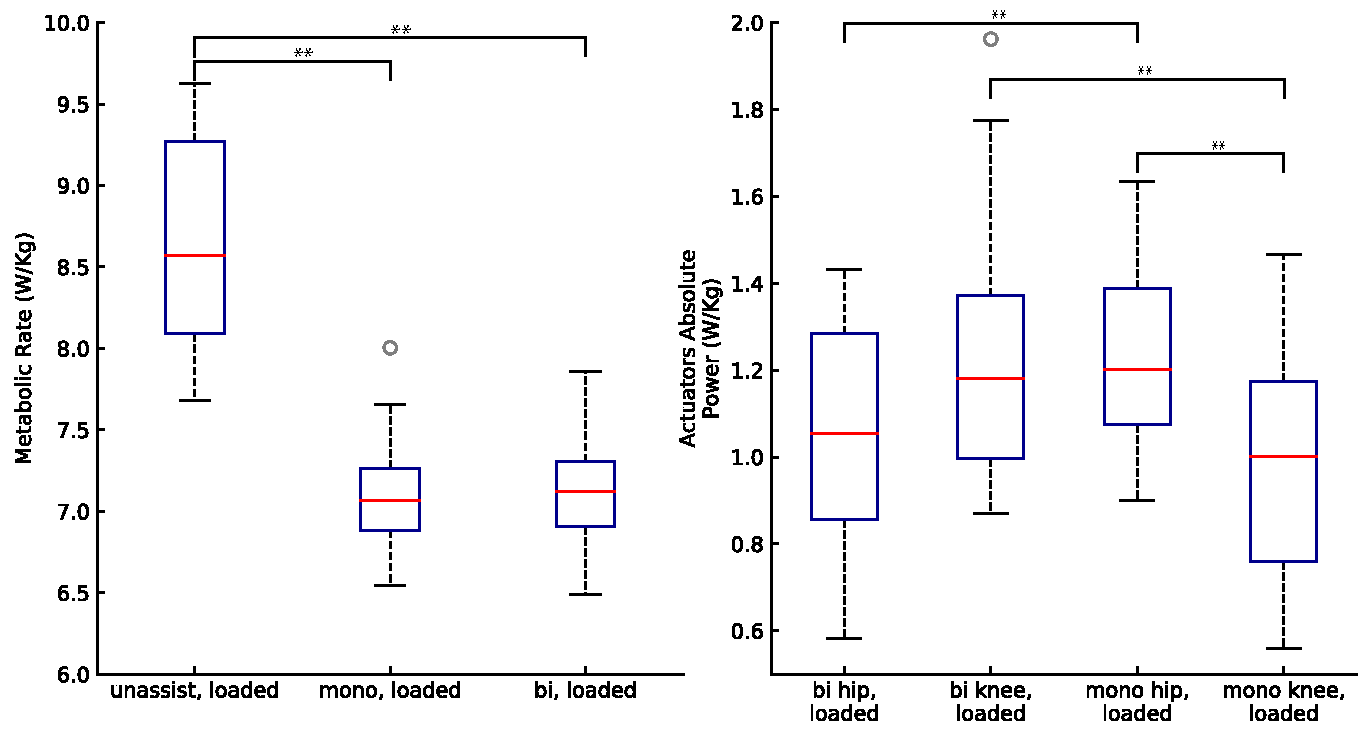
\includegraphics[width=\linewidth]{Case_Studies/LoadedMono04_LoadedBi16/PaperFigure_BoxPlot.pdf}
	\vspace{1mm}
	\caption{\small{\textbf{Assistive devices power consumption and its effect on the metabolic rate.} The power consumptions of assistive devices and their effect on whole-body metabolic rate of the subjects walking at self-selected speed while carrying a heavy load. Asterisks indicate statistically significant differences ( 7 subjects, 3 trails, Tukey Post-hoc, $P < 0.05$).}}
	\label{Fig_Case01_Energy_Plot}
\end{figure*}
The metabolic rate of assisted subjects with biarticular and monoarticular devices shows that there is no significant difference between the amount of assistance delivered by these devices, which was expected from the Pareto front. While the total power consumptions of these two devices are practically identical on the Pareto front, the power rate of hip and knee between biarticular and monoarticular devices are statistically significantly different as it is represented in figure \ref{Fig_Case01_Energy_Plot}. This difference indicates that while they have the devices deliver an equal amount of assistance to the subjects with a heavy load, their assistance strategies are different, which can be illuminated by analyzing the profiles of actuators.\\
\begin{figure*}[ht]   
	\centering
	\includegraphics[width=\linewidth]{Case_Studies/LoadedMono04_LoadedBi16/PaperFigure_Profiles.pdf}
	\vspace{1mm}
	\caption{{\small\textbf{Assistive devices torque and power profiles.} The actuator torque and power for subjects carrying heavy load (dark blue) , and net joint power profile for \textit{loaded} (black) condition are shown for each actuator of the devices. The curves are averaged over 7 subjects with 3 trials and normalized by subject mass; shaded regions around the mean profile indicate standard deviation of the profile.}}
	\label{Fig_Case01_Torque_Power_Profiles}
\end{figure*}
\begin{figure*}[ht]   
	\centering
	\includegraphics[width=\linewidth]{Case_Studies/LoadedMono04_LoadedBi16/RMSE.pdf}
	\vspace{1mm}
	\caption{\small{\textbf{Assistive devices torque and power and muscles generated moment profiles root mean square error. } The root mean square error between actuators of biarticular and monoarticular devices and the muscles generated moment of subjects assisted by these devices.}}
	\label{Fig_Case01_RMSE}
\end{figure*}
The overall trend between torque profiles of the monoarticular and biarticular devices is similar, which can be seen in figure \ref{Fig_Case01_Torque_Power_Profiles} qualitatively, and root mean square error between the profiles during the whole gait cycle can also proof this quantitatively claim as shown in figure \ref{Fig_Case01_RMSE}. The detailed analysis of the gait cycle shows that the main difference between torque profiles of hip actuators is occurring during the stance phases and monoarticular deliver more hip extension torque than the biarticular device, especially during the mid-stance and terminal-stance phases (Fig. \ref{Fig_Case01_Torque_Power_Profiles} and \ref{Fig_Case01_RMSE}). Although the difference between profiles of hip actuators follow similar trajectories during the swing phase, the terminal-swing phase of these actuators is considerably different in which monoarticular deliver extension while biarticular provide flexion torque to the joint.\\
Although the biarticular and monoarticular knee actuators have an almost identical trajectory during the swing phase as their RMSE also shows in figure \ref{Fig_Case01_RMSE}, there are some significant differences between these two actuators during the stance phases. While the biarticular knee actuator opposes with the torque generated by muscles around the knee joint during all stance phase, the monoarticular knee actuator assists the knee muscles generated torque during the loading response and mid-stance phases.\\ These remarkable differences between torque profiles of two devices affect the torque trajectories generated by muscles around the knee and hip joints, indicating muscular activation differences between subjects assisted by monoarticular and biarticular exoskeletons, nevertheless, according to the root mean square error between hip and knee muscles generated torque trajectories, the differences are not substantial except on the loading phase of the knee joint.\\
The comparison between the muscular activation of the {\it loaded} subjects assisted by ideal devices and constrained devices indicates substantial differences in some muscles. The activation of rectus femoris and psoas as two primary muscles on the hip and knee are considerably different between these two conditions, which can also explain the significant part of the difference between the muscle activations. This difference is not only between the ideal and constrained device but also the constrained biarticular, and monoarticular exoskeletons have a different impact on these two muscles (\nameref{S2_Fig}), which can roughly explain the variation between the muscles generated moment. Another remarkable difference between the ideal and constrained devices can be seen in gastrocnemius medial head muscle, where the activation of this muscle has been increased during the loading response to terminal stance phases. Since the activation of the gastrocnemius muscle increased, it can provide more moment on the ankle as well, and the activation of the soleus does not need to be increased considerably to compensate for the inadequacy of the moment generated by gastrocnemius.
The muscular activation of subjects assisted by monoarticular and biarticular constrained devices are not limited to rectus femoris and psoas muscles, but the other representative muscles show some differences as it is shown in the figure in \nameref{S2_Fig} nevertheless, the differences between them are not as considerable as rectus femoris and psoas muscles.\\
Unlike the moment profiles of devices where the difference was significant only in some specific phases, the power profiles of the biarticular and monoarticular devices have significant differences as it is shown qualitatively and quantitatively in figure \ref{Fig_Case01_Torque_Power_Profiles} and \ref{Fig_Case01_RMSE} respectively. The difference between the power profiles of these two dives is more notable in the knee actuator in which the devices follow different trajectories during the gait cycle. Similar to the knee actuators, the hip actuators also have roughly different power profiles, and their maximum power consumptions occur in two completely different phases, similar to the knee actuators.  The difference between the trajectories and magnitudes of the power profiles also can explain the statistically significant difference observed between the monoarticular and biarticular exoskeletons (Fig.\ref{Fig_Case01_Energy_Plot}).\\
Unlike the moment profiles of devices where the difference was significant only in some specific phases, the power profiles of the biarticular and monoarticular devices have significant differences as it is shown qualitatively and quantitatively in figure \ref{Fig_Case01_Torque_Power_Profiles} and \ref{Fig_Case01_RMSE} respectively. The difference between the power profiles of these two dives is more notable in the knee actuator in which the devices follow different trajectories during the gait cycle. Similar to the knee actuators, the hip actuators also have roughly different power profiles, and their maximum power consumptions occur in two completely different phases, similar to the knee actuators.  The difference between the trajectories and magnitude of the power profiles also can explain the statistically significant difference observed between the monoarticular and biarticular exoskeletons.\\
Although the selected monoarticular and biarticular exoskeletons have the same effect on the metabolic rate of {\it loaded} subjects, it is already shown that their assistive actuator configurations are different which resulted in significantly different power rate of actuators. This difference in the configuration of their actuators affects their mechanical design, especially their required gear train and reflected inertia consequently. We employed the developed modified augmentation factor to assess the performance of the biarticular and monoarticular exoskeletons under the effect of device inertial properties. The computed modified augmentation factor for monoarticular and biarticular was 0.66 $\pm$ 1.00 and  1.98 $\pm$ 0.71 W/kg, which indicates that both exoskeletons would be able to deliver assistance to the subjects even under inertial properties of devices causing more metabolic burden on the subject. Additionally, the MAF shows that biarticular device has superior performance than monoarticular exoskeleton and the reason for this issue embedded on the mass distribution and gear train of the monoarticular device. The inertia calculations show the device has practically three times more inertia on the thigh than the biarticular device and, according to Eqn.\eqref{Eqn_MAF} and the inertia location factor of the thigh, the effect of inertia on the thigh is expensive in terms of the metabolic rate increase which results in a lower MA factor for the monoarticular exoskeleton.\\
Studying this specific case of monoarticular and biarticular devices proves the devices with the same total power consumption can have different power consumption in different joints. Additionally, it is shown that the optimal devices with the same performance can follow different moment and power profiles, even under kinematic similarities due to the arrangement of actuators. Although the devices were selected from the ideal Pareto front with the same performance, employing the modified augmentation factor for the monoarticular and biarticular devices with different mass and inertia characteristics indicated the superior performance of the biarticular device. It emphasizes the discussion held in the Mass, inertia, and regeneration effects section that biarticular device could deliver the same amount of assistance to the subjects more effectively than the monoarticular configuration.\\
\subsubsection*{Case 2: Devices Performance in \textit{\textit{noload}} Condition}
In the second case study, we selected two devices with different power consumptions and the same effect on the metabolic rate of subjects walking without any extra load, which are shown with {\it "Cb" } and {\it "Ba" } on the biarticular and monoarticular Pareto front of the {\it noload} condition. Although the total performance trade-off of these two biarticular and monoarticular devices are different in mean values, the statistical tests on the mean absolute power consumption of actuator showed no statistically significant difference between actuators of the monoarticular and biarticular exoskeletons.
\begin{figure*}[ht]   
	\centering
	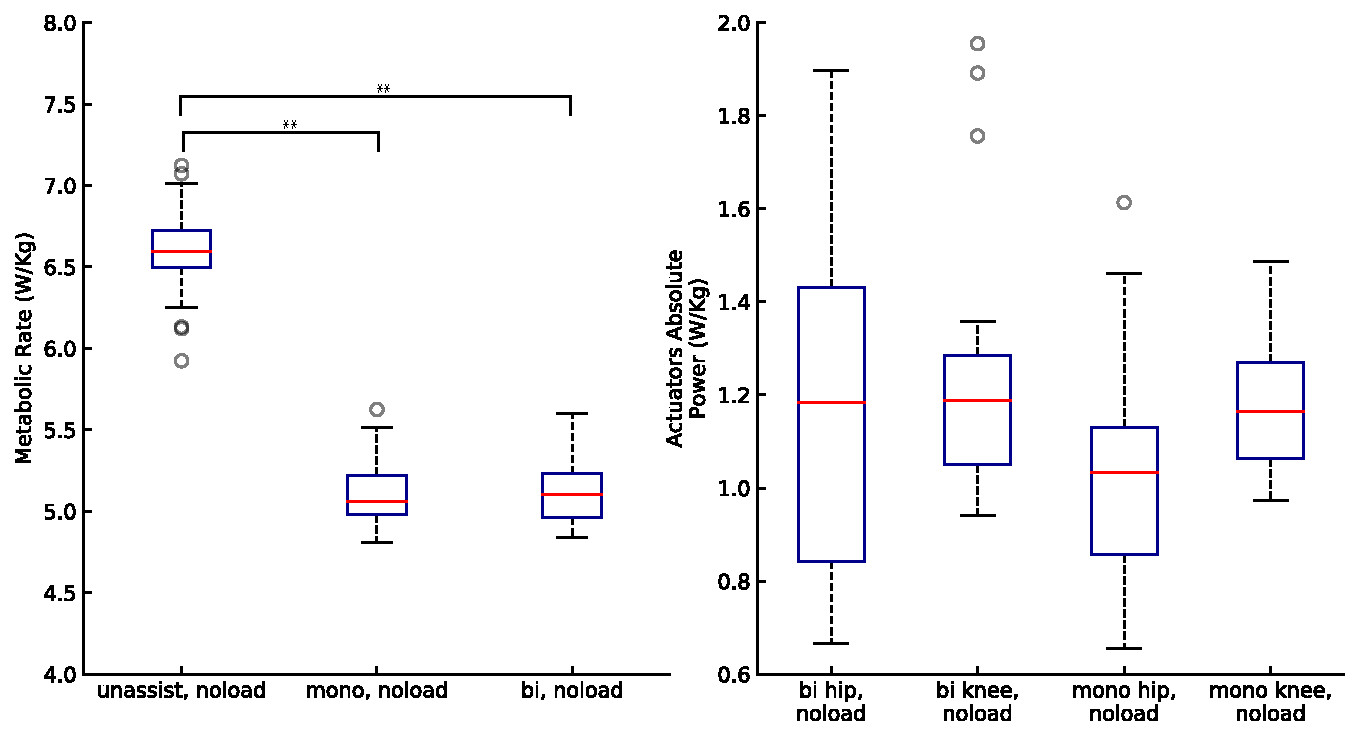
\includegraphics[width=\linewidth]{Case_Studies/NoloadMono06_NoloadBi12/PaperFigure_BoxPlot.pdf}
	\vspace{1mm}
	\caption{\small{\textbf{Assistive devices power consumption and its effect on the metabolic rate.} The power consumptions of assistive devices and their effect on whole-body metabolic rate of the subjects walking at self-selected speed without any additional load. Asterisks indicate statistically significant differences ( 7 subjects, 3 trails, Tukey Post-hoc, $P < 0.05$).}}
	\label{Fig_Case02_Energy_Plot}
\end{figure*}
\begin{figure*}[ht]   
	\centering
	\includegraphics[width=\linewidth]{Case_Studies/NoloadMono06_NoloadBi12/PaperFigure_Profiles.pdf}
	\vspace{1mm}
	\caption{{\small\textbf{Assistive devices torque and power profiles.} The actuator torque and power for subjects carrying heavy load (dark blue) , and net joint power profile for \textit{loaded} (black) condition are shown for each actuator of the devices. The curves are averaged over 7 subjects with 3 trials and normalized by subject mass; shaded regions around the mean profile indicate standard deviation of the profile.}}
	\label{Fig_Case02_Torque_Power_Profiles}
\end{figure*}
\begin{figure*}[ht]   
	\centering
	\includegraphics[width=\linewidth]{Case_Studies/NoloadMono06_NoloadBi12/RMSE.pdf}
	\vspace{1mm}
	\caption{\small{\textbf{Assistive devices torque and power and muscles generated moment profiles root mean square error. } The root mean square error between actuators of biarticular and monoarticular devices and the muscles generated moment of subjects assisted by these devices.}}
	\label{Fig_Case02_RMSE}
\end{figure*} 
The power consumption of hip actuators in both exoskeletons had a high within-subject deviation, as it is shown in figure \ref{Fig_Case02_Energy_Plot}, which may explain the absence of a statistically significant difference between the actuators.  Additionally, the metabolic rate of subjects assisted with monoarticular and biarticular devices has no significant difference; still, the metabolic rate reduction caused a significant difference between the unassisted and assisted subjects, as represented in figure \ref{Fig_Case02_Energy_Plot}. \\
The analysis of moment profiles of assistive devices in the {\it noload} condition shows that the differences between these two devices are similar to the difference of biarticular and monoarticular devices in the {\it loaded} circumstance which is represented in figure \ref{Fig_Case02_Torque_Power_Profiles}. Nevertheless, the variations of moment generated by muscles of assisted subjects are negligible in {\it noload} condition (Fig. \ref{Fig_Case02_RMSE}), which signals identical muscular activation of subjects assisted with these exoskeletons. Unlike the moment profiles, the power profiles of the devices are different in {\it noload} condition, unlike the moment patterns. It can be seen from the power profiles that devices follow notably different trajectories during a gait cycle to deliver assistance to the subjects and these profiles in the hip actuators, similar to the knee actuators, have the highest contrast during the pre-swing phase according to their RMS error shown in figure \ref{Fig_Case02_RMSE}.\\
Despite the large variation between the power consumption of the devices and the absence of significant difference among their actuators, employing the modified augmentation factor indicates the remarkably different performance for monoarticular and biarticular exoskeletons on delivering assistance to the subjects. The selected devices have a different design in the actuators in which the biarticular device can provide maximum 50 and 60 N-m/kg torque in hip and knee actuators respectively; yet, the maximum providable moments in the hip and knee actuators of the monoarticular device are 60 and 70 N-m/kg respectively. The computation of MAF under described configurations of devices resulted in 1.57$\pm$0.72 W/kg and 0.42$\pm$0.85 for biarticular and monoarticular devices indicating the better performance of the biarticular device similar to the first case. The performance of these two devices can also be discussed based on the Pareto front of devices under inertia and mass effect shown in figure \ref{Fig_Paretofronts_Mass_Regeneration_Effect}. According to this analysis ( Fig. \ref{Fig_Paretofronts_Mass_Regeneration_Effect}), the studied configuration of the monoarticular device became a nondominant solution in Pareto simulations under the inertial properties of devices, while the chosen biarticular device could maintain its efficiency under the negative effect of its inertial properties on the metabolic rate of subjects. This analogy between the Pareto front with devices inertial properties effect consideration and MAF can also confirm the extension of the augmentation factor.\\
Studying specific optimal monoarticular and biarticular exoskeletons in two load conditions which were chosen from the Pareto fronts show that the even though the devices have practically the same performance in the optimal trade-off between the device total power consumption and metabolic cost reduction curves, their provided moment during a gait cycle has considerable differences which can have a different effect on the muscular activation of assisted subjects as well. These two case studies also show that the power profiles of monoarticular and biarticular devices are considerably different, though they have a similar total power consumption.\\
The study on the performance of selected devices in both loading conditions by developed MAF factor supports the discussion held on the "Mass, inertia and regeneration effects" section on the effect of the mechanical design on the performance of devices and also showed that the performance of the monoarticular exoskeleton highly affected with the inertial properties of the device. Although the mechanical design of a biarticular device can be complicated, its performance under the device inertial properties seems promising in both loading conditions according to the performance of studied cases (MAF value). The studied cases and general Pareto front of monoarticular device under its inertial characteristics effect show that the monoarticular device needs to be designed thoughtfully to reduce the effect of inertia and mass effect of the device on the metabolic burden of subjects complicating the design procedure and ignoring the mechanical design may result in delivering no assistance to the subject or increasing their metabolic burden. Even if the device with poor mechanical design can deliver assistance to the subjects, it will be costly in terms of power consumption. 
\subsubsection*{Case 3: Biarticular Exoskeleton Performance}
To study how the performance of the biarticular exoskeleton changes by loading subjects with a heavy weight on torso more specifically, we chose two cases in which the biarticular exoskeletons had the same effect on the metabolic rate of subjects in one case, and they had the same power consumption in another case.\\ 
\begin{figure*}[th!]
	\centering
	\subfloat[\small{Biarticular exoskeleton with the same effect on the metabolic consumption of subjects}]{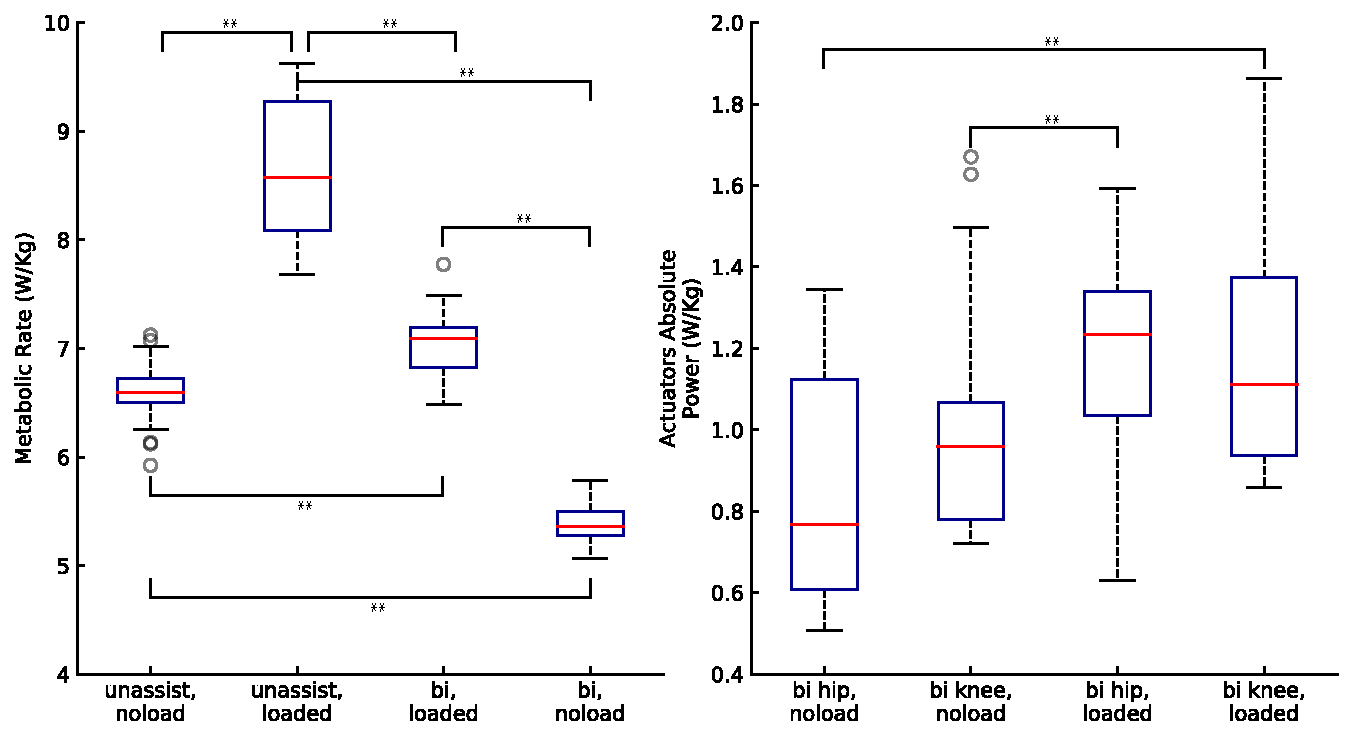
\includegraphics[width=\linewidth]{Case_Studies/NoloadBi23_LoadedBi12/PaperFigure_BoxPlot.pdf}
		\label{Fig_Case03_Energy_Plot_SameMetabolicConsumption}}
	\hfil
	\subfloat[\small{Biarticular exoskeleton with the same total power consumptions }]{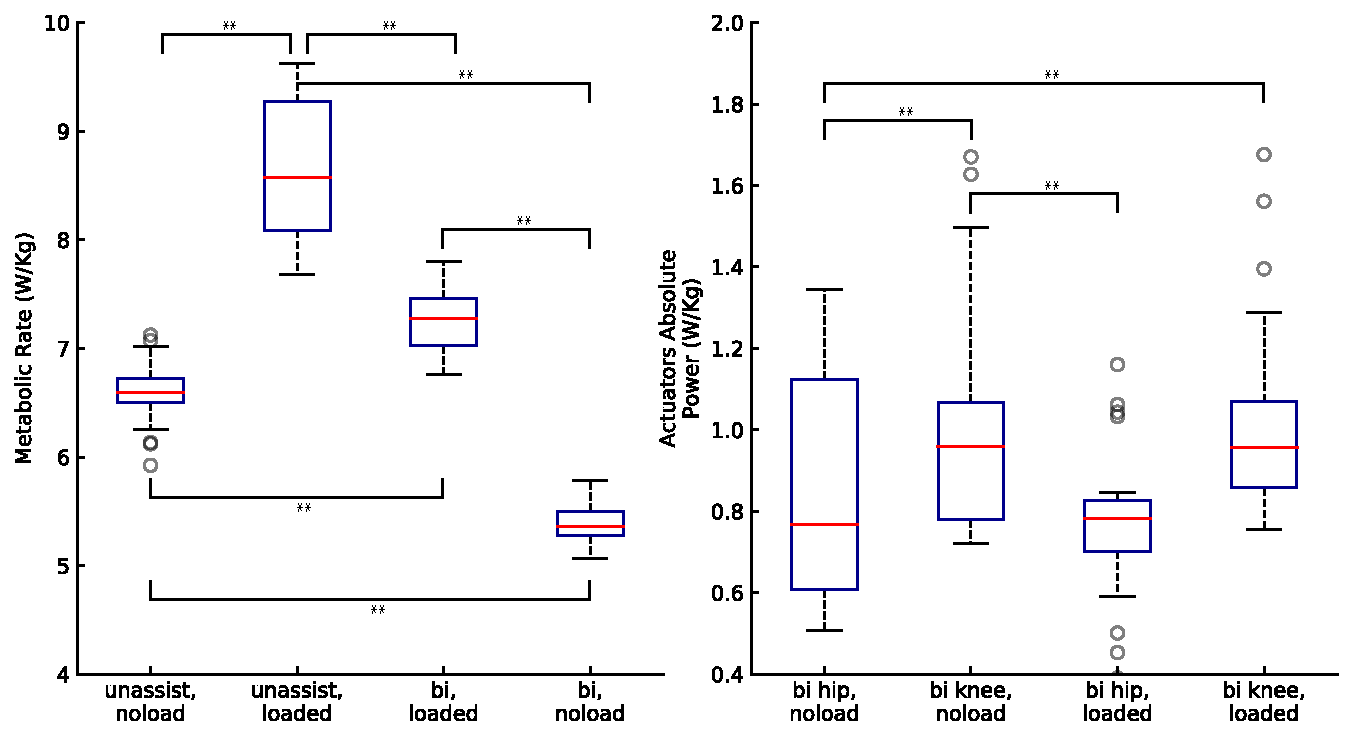
\includegraphics[width=\linewidth]{Case_Studies/NoloadBi23_LoadedBi23/PaperFigure_BoxPlot.pdf}
		\label{Fig_Case03_Energy_Plot_SamePowerConsumption}}
	\vspace{2mm}
	\caption{\small{\textbf{Biarticular exoskeleton power consumption and its effect on the metabolic rate in different load conditions.} The power consumptions of biarticular exoskeleton and their effect on whole-body metabolic rate of the subjects walking at self-selected speed in both {\it loaded} and {\it noload} condition. Asterisks indicate statistically significant differences ( 7 subjects, 3 trails, Tukey Post-hoc, $P < 0.05$).}}
	\label{Fig_Case03_Energy_Plot}
\end{figure*}
\begin{figure*}[ht!]
	\centering
	\subfloat[\small{Biarticular exoskeleton with the same effect on the metabolic consumption of subjects}]{\includegraphics[width=\linewidth]{Case_Studies/NoloadBi23_LoadedBi12/RMSE.pdf}
		\label{Fig_Case03_RMSE_SameMetabolicConsumption}}
	\hfil
	\subfloat[\small{Biarticular exoskeleton with the same total power consumptions }]{\includegraphics[width=\linewidth]{Case_Studies/NoloadBi23_LoadedBi23/RMSE.pdf}
		\label{Fig_Case03_RMSE_SamePowerConsumption}}
	\vspace{1mm}
	\caption{\small{\textbf{Biarticular exoskeleton torque and power and muscles generated moment profiles root mean square error in different load conditions.} The root mean square error between actuators of the biarticular exoskeleton and the muscles generated moment of subjects assisted by this device {\it loaded} and {\it noload} conditions.}}
	\label{Fig_Case03_RMSE}
\end{figure*}
The selected configuration of the biarticular exoskeleton in {\it noload} condition is $"Ec"$ with 30 and 50 N-m/kg peak torque in the hip and knee actuators, and it was compared to the same configuration (i.e., $"Ec"$) in  {\it loaded} condition where they had practically the same power consumption according to figure \ref{Fig_Main_Paretofronts}. For conducting the comparison with the likewise metabolic burden reduction, the same configuration of {\it noload} condition (i.e., $"Ec"$) was compared to the biarticular exoskeleton with 50 and 60 N-m/kg peak torque in the hip and knee actuators represented by $"Cb"$ on the Pareto front of the {\it loaded} biarticular exoskeleton.\\
The comparisons of the metabolic rate of assisted subjects by the biarticular device in two similar metabolic reduction and power consumption conditions have been represented in figure \ref{Fig_Case03_Energy_Plot}. The metabolic rate of subjects in both conditions shows that even though the metabolic rate of loaded subjects reduce considerably, there is a statistically significant difference between subjects walking normally and subjects assisted by the biarticular device in the {\it loaded} condition. The power consumption of the hip actuator, as well as the knee actuators in both loading conditions, showed no significant difference when the selected device was consuming a similar amount of power in both loading conditions; nevertheless, we observed a significant difference between the knee and hip actuators in different load conditions as shown in figure \ref{Fig_Case03_RMSE}\subref{Fig_Case03_RMSE_SamePowerConsumption}. Additionally, a similar performance in power consumption of  two different configurations of the biarticular exoskeleton delivering a similar amount of assistance in different load conditions has been observed, which is represented in figure \ref{Fig_Case03_RMSE}\subref{Fig_Case03_RMSE_SameMetabolicConsumption}.\\
The absence of a significant difference between two devices with different configurations and different load conditions can facilitate designing a battery with a robust performance in different load conditions, and also this performance can help to have a general mechanical design for an exoskeleton to assist subjects in different load and assistance level conditions. Nevertheless, the high deviations and outliers of power consumption indicate high contrast within subjects that can complicate obtaining general power profiles for the device.\\
The performance assessment of the same biarticular configuration in two different load conditions by employing MAF showed that the performance of the biarticular exoskeleton in {\it loaded} condition was improved (1.40$\pm$0.80 W/kg) in comparison with the  {\it noload} condition where MAF was 1.01$\pm$0.70 W/kg. Although the increase in the positive power of the device in {\it loaded} condition was expected, MAF improvement shows that this increase in positive power was delivered to the subjects effectively. In the meanwhile, comparing the devices with the same effect on the metabolic cost reduction of subjects in different load conditions showed superior performance of the biarticular device in the {\it loaded} in which devices in {\it loaded} and {\it noload} circumstances had  2.08$\pm$0.69 and 1.01 $\pm$0.69 W/kg MAF value which can indicate inefficiency of noload device power profiles in general.\\
The quantitative along with the qualitative analyses of power and moment profiles between pair of devices in defined comparison cases not only show a moderate variation between the torque profiles of the compared biarticular device but also the power profiles have considerably low diversity in different load conditions as it is shown in figure \ref{Fig_Case03_RMSE}\subref{Fig_Case03_RMSE_SameMetabolicConsumption}, \ref{Fig_Case03_RMSE}\subref{Fig_Case03_RMSE_SamePowerConsumption}, and figure in \nameref{S3_Figure} supporting our claims on the high resemblance between profiles of the biarticular exoskeletons in loaded and noload conditions. As it is shown in figure in \nameref{S3_Figure}, the difference between the power and moment profiles of pair of devices in {\it load} and {\it noload} conditions are practically limited to the magnitude and timing based on the toe-off difference except on the pre-swing and initial-swing phases of knee profiles where the trajectories have rough differences between biarticular devices with the same effect on the metabolic power consumption of assisted subjects.
\subsubsection*{Case 4: Monoarticular Exoskeleton Performance} 
\begin{figure*}[ht!]
	\centering
	\subfloat[\small{Monoarticular exoskeleton with the same effect on the metabolic consumption of subjects}]{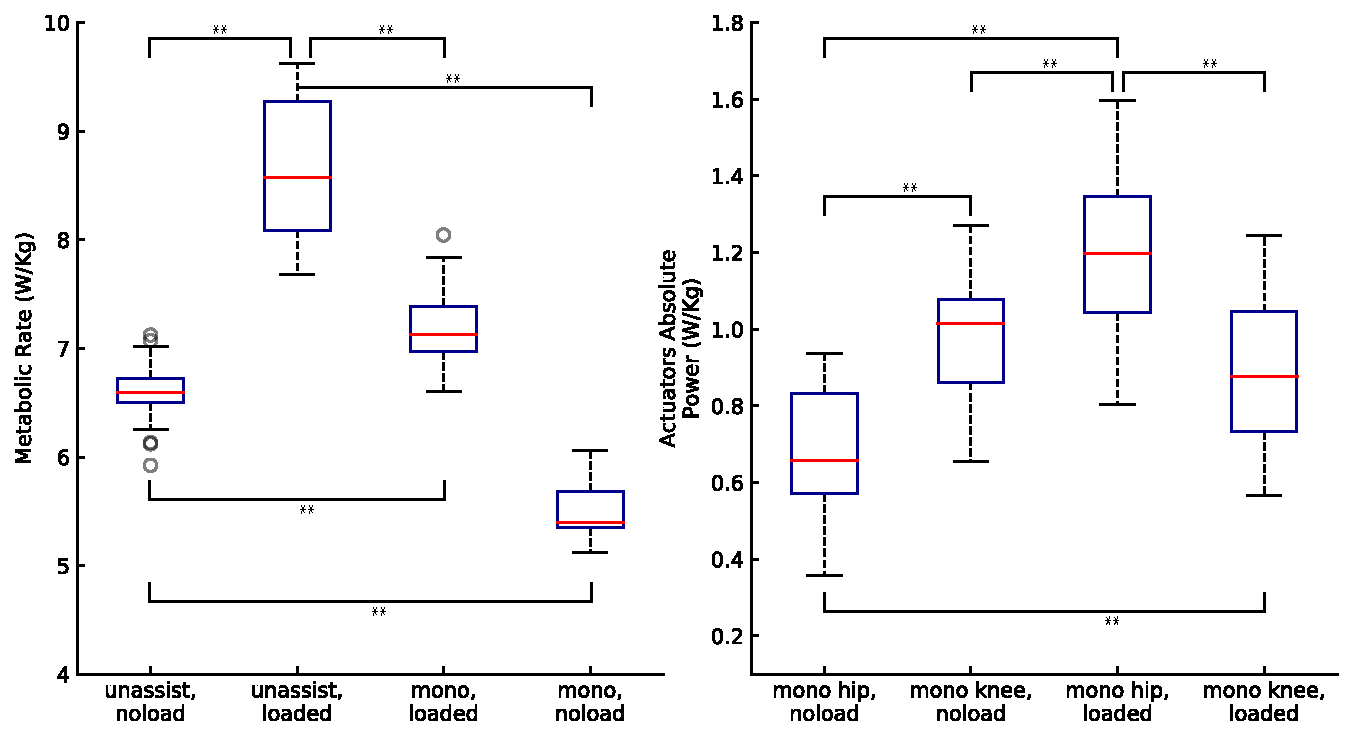
\includegraphics[width=\linewidth]{Case_Studies/NoloadMono25_LoadedMono05/PaperFigure_BoxPlot.pdf}
		\label{Fig_Case04_Energy_Plot_SameMetabolicConsumption}}
	\hfil
	\subfloat[\small{Monoarticular exoskeleton with the same total power consumptions }]{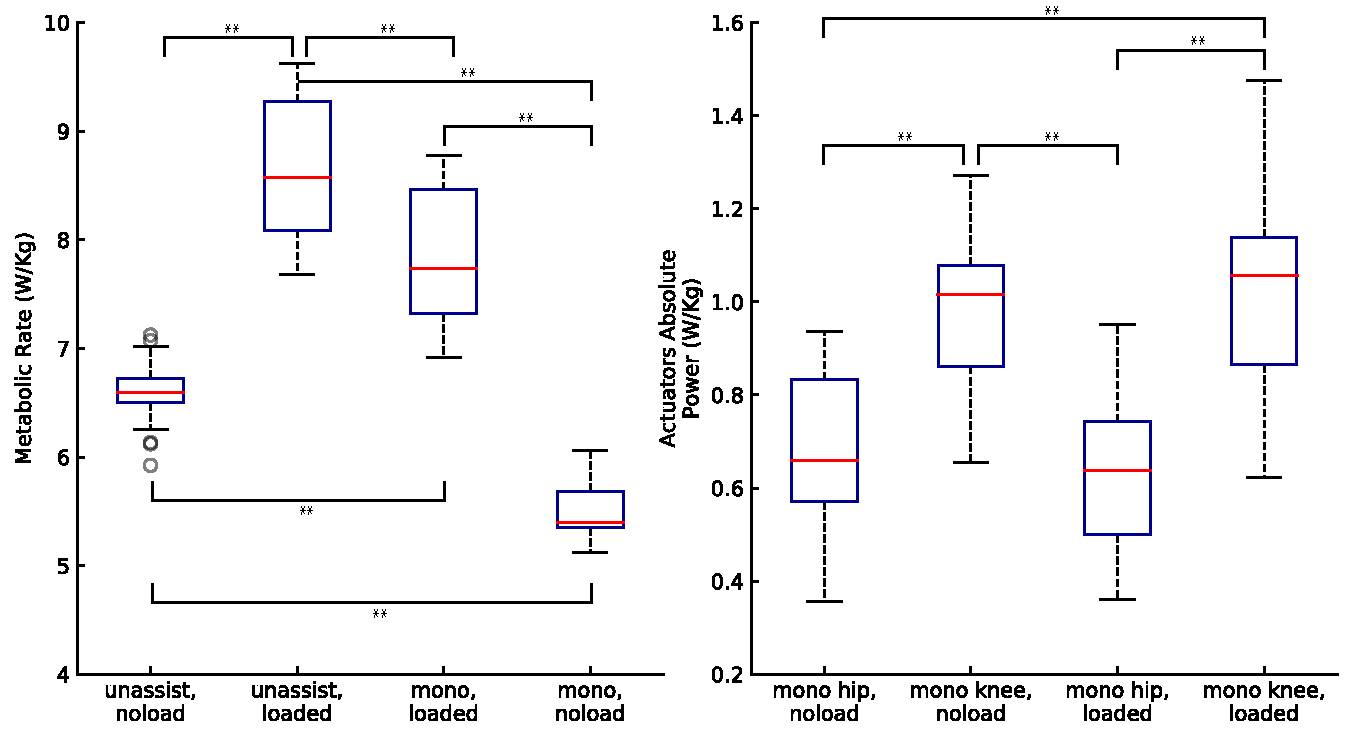
\includegraphics[width=\linewidth]{Case_Studies/NoloadMono25_LoadedMono25/PaperFigure_BoxPlot.pdf}
		\label{Fig_Case04_Energy_Plot_SamePowerConsumption}}
	\vspace{1mm}
	\caption{\small{\textbf{Monoarticular exoskeleton power consumption and its effect on the metabolic rate in different load conditions.} The power consumptions of biarticular exoskeleton and their effect on whole-body metabolic rate of the subjects walking at self-selected speed in both {\it loaded} and {\it noload} condition. Asterisks indicate statistically significant differences ( 7 subjects, 3 trails, Tukey Post-hoc, $P < 0.05$).}}
	\label{Fig_Case04_Energy_Plot}
\end{figure*}
\begin{figure*}[ht!]
	\centering
	\subfloat[\small{Monoarticular exoskeleton with the same effect on the metabolic consumption of subjects}]{\includegraphics[width=\linewidth]{Case_Studies/NoloadMono25_LoadedMono05/RMSE.pdf}
		\label{Fig_Case04_RMSE_SameMetabolicConsumption}}
	\hfil
	\subfloat[\small{Monoarticular exoskeleton with the same total power consumptions }]{\includegraphics[width=\linewidth]{Case_Studies/NoloadMono25_LoadedMono25/RMSE.pdf}
		\label{Fig_Case04_RMSE_SamePowerConsumption}}
	\vspace{1mm}
	\caption{\small{\textbf{Monoarticular exoskeleton torque and power and muscles generated moment profiles root mean square error in different load conditions.} The root mean square error between actuators of the biarticular exoskeleton and the muscles generated moment of subjects assisted by this device {\it loaded} and {\it noload} conditions.}}
	\label{Fig_Case04_RMSE}
\end{figure*}
The same analyses on the biarticular exoskeleton in different load conditions, which was discussed in the previous case study,  were performed on the monoarticular exoskeleton to get an in-depth insight into this device. To conduct the comparisons between a pair of monoarticular devices with a similar effect on the metabolic cost or with similar power consumption, we chose the $"Ee"$ configuration of monoarticular in loaded and noload conditions and $"Ae"$ monoarticular exoskeleton from the Pareto front of monoarticular in the loaded condition.The selected $"Ee"$ and $"Ae"$ configurations have 30 and 30N-m/kg and 70 and 30 N-m/kg peak torque constraints on the pair of hip and knee actuators.\\
The comparison of actuators power consumption between $"Ae"$ {\it loaded} and $"Ee"$ {\it noload}, which have a similar metabolic cost reduction, showed a notable increase in power consumption of the {\it loaded} hip actuator. Despite the reduction in the knee power consumption of {\it loaded} knee actuator, the difference between the pair knee actuators was not significant. One of the observed critical issues was that even though the within-subject variation of monoarticular devices was generally low, the divergence of actuators power consumption between the load condition and between the configurations was considerably high. As it is shown in figure \ref{Fig_Case04_Energy_Plot}\subref{Fig_Case04_Energy_Plot_SameMetabolicConsumption} along with figure \ref{Fig_Case04_Energy_Plot}\subref{Fig_Case04_Energy_Plot_SamePowerConsumption}, while the power consumption of knee actuator in the low torque availability (i.e., $Ee$) was higher than the hip actuator, this was changed in higher torque constraints in which the hip became dominant power consumer that indicates considerable changes in the power profile of monoarticular device in different arrangements of its actuators.\\
The metabolic rate of the compared pairs of monoarticular devices has been shown in figure \ref{Fig_Case04_Energy_Plot}\subref{Fig_Case04_Energy_Plot_SameMetabolicConsumption} and \ref{Fig_Case04_Energy_Plot}\subref{Fig_Case04_Energy_Plot_SamePowerConsumption} that showed similar behavior observed in the previous case study; yet, it is noteworthy to mention the significant difference between the impact of $"Ee"$ device on the metabolic burden reduction of subjects in different loading conditions that we did not observe in the biarticular case according to the Pareto front of a device in different load conditions as shown in figure\ref{Fig_Main_Paretofronts}. These high deviations in both defined performance criteria can complicate obtaining a general exoskeleton that can deliver different levels of assistance with efficient power consumption.\\
The pair of devices selected for conducting the comparisons were evaluated by the modified augmentation factor to assess their performance under the mass and inertia effect. Unlike the other case studies in which all evaluated biarticular and monoarticular devices were delivering a positive power to the human musculoskeletal system, the monoarticular exoskeletons evaluated in this case study both were causing an increase in the metabolic burden of subjects according to MAF performance factor. The modified augmentation factor of the monoarticular device with 30 N-m/kg peak torque constraints in both hip and knee actuators showed -0.20 $\pm$ 0.43 W/kg in the {\it noload} condition while it was increased to -0.15 $\pm$ 0.56 W/kg when subjects were loaded.These MAF values of the $"Ee"$ monoarticular device represent a high variation of device effect on the subjects and improvement of the device performance by loading subjects, which was also observed in the biarticular exoskeleton. Even with the improvement of device performance in the loaded condition, the device in both load conditions would cause subjects to consume more power due to wearing these devices. The same analysis on the monoarticular device $"Ae"$ configuration ( 70  N-m/kg hip 30 N-m/kg knee) in  {\it loaded} condition showed relative improvement compared to the $"Ee"$ device.\\
According to the MAF, the monoarticular exoskeleton require large torque capacity to deliver assistance to the subjects, and this observation is in contraction with our earlier claim about the monoarticular device in the {\it noload}  condition under the inertial properties effect of devices. According to the slope of Pareto front of monoarticular device under the devices inertial properties effect, we claimed that it might be beneficial to keep the torque capacity of the monoarticular exoskeleton more moderate, yet, we observe in this case study that the monoarticular device cannot inject positive power to the human musculoskeletal system in low torque capacity, and this contraction might be due to the differences between definitions of MAF and Pareto fronts under inertial effect which demands experimental justifications of defined performance criteria.\\
Although there are some quantitative divergences between the defined performance metrics, both Pareto front and MAF revealed the remarkably weak performance of monoarticular under device mass and inertia effect consideration. The MAF, along with Pareto front, supports our previous discussion regarding the monoarticular exoskeleton design and control and shows the necessity of inertia and gravity compensation for improving the efficiency of this device, which will lead to complex control architectures introducing several new challenges such as stability analysis, fundamental limitations, and other difficulties discussed in detail earlier.\\
The moment and power profiles of the selected monoarticular exoskeleton did not show a similar resemblance we observed in the biarticular device between the pair of actuators. The hip actuators of devices with the same metabolic reduction effect follow completely different trajectories, and it is not surprising that their power profiles have significant differences. Although the moment profiles of the knee actuators had a higher resemblance than the hip actuators, their power profiles showed relatively different paths during pre-swing and initial swing phases. The comparison of profiles in the same device ( i.e., $Ee$) in different load conditions showed a considerable divergence between the moment and power profiles of hip actuator after the mid-stance phase of the gait cycle and their maximum difference have occurred during pre-swing and initial swing phases. The knee actuators showed a similar performance we already observed in another comparison condition in which even though the torque profiles of knee actuator in different load conditions were almost the same, their power profiles have remarkable differences during pre-swing and initial swing phases. These described moment and power profiles and their quantitative differences using RMSE in both comparison cases have been represented in the figure in \nameref{S4_Figure} and figure \ref{Fig_Case04_RMSE}.\\
These variations on the profiles of the monoarticular device were already observed on the analysis of optimal devices torque and power profiles shown in figure \ref{Fig_Paretofronts_Torque_Profiles} and \ref{Fig_Paretofronts_Power_Profiles}. These case studies confirm our discussion about monoarticular exoskeleton in which we claim that obtaining a generic control profile for this device would be challenging and also the optimal battery design under its life and weight considerations, as optimality criteria, highly dependent on the selected configuration and a generic battery would not perform optimally for all devices.
\end{document}
